\section{Descriptive statistics}\label{sec: result_table}

\setcounter{figure}{0}    
\setcounter{table}{0}
\renewcommand\thetable{\thesection.\arabic{table}}  
\renewcommand\thefigure{\thesection.\arabic{figure}}  

Below, we show detailed tables and figures of descriptive statistics collected from the usability study.

\subsection*{Task completion}

\aptLtoX[graphic=no,type=html]{ \begin{table}[H]
    \centering
    \begin{tabular}[t]{l|r r r r}
        & Task C1 & Task C2 & Task E1 & Task E2 \\\hline
        \textit{FFL}     &3&2&0&1\\
        \LaTeX  &2&1&1&8
    \end{tabular}
    \Description{Table. Each row corresponds to an interface, and each column corresponds to a task that was completed with that interface. Cells contain counts of participants who completed the task with that interface.}
    \vspace{1ex}
    \captionof{table}{Counts of participants who did not complete timed tasks (each count is out of 14 participants).}
    \label{tab:count_fail_task}
 \end{table} }{ % \begin{table}[H]
\begin{center}
    \centering
    \begin{tabular}[t]{l|r r r r}
        & Task C1 & Task C2 & Task E1 & Task E2 \\\hline
        \textit{FFL}     &3&2&0&1\\
        \LaTeX  &2&1&1&8
    \end{tabular}
    \Description{Table. Each row corresponds to an interface, and each column corresponds to a task that was completed with that interface. Cells contain counts of participants who completed the task with that interface.}
    \vspace{1ex}
    \captionof{table}{Counts of participants who did not complete timed tasks (each count is out of 14 participants).}
    \label{tab:count_fail_task}
\end{center}
% \end{table}
 } 


\aptLtoX[graphic=no,type=html]{ \begin{table}[H]
    % \centering
    \resizebox{\linewidth}{!}{
        \begin{tabularx}{1.07\linewidth}{X|c c c c c c c c}
            Time&\multicolumn{2}{c}{Task C1}&\multicolumn{2}{c}{Task C2}&\multicolumn{2}{c}{Task E1}&\multicolumn{2}{c}{Task E2} \\
            (s)&\textit{FFL}&\LaTeX&\textit{FFL}&\LaTeX&\textit{FFL}&\LaTeX&\textit{FFL}&\LaTeX \\\hline
            $\bar{x}$&253.3&242.8&258.1&229.2&157.3&206.0&223.4&350.4\\
            $\sigma$&97.65&101.1&98.6&95.8&66.4&81.3&87.5&68.1
        \end{tabularx}
    }\Description{Table of task completion times, in seconds, by interface-task pair (measured in seconds). Task C1 with FFL, mean: 253.3, standard deviation: 97.65; with LaTeX, mean: 242.8, standard deviation: 101.1. Task C2, with FFL, mean: 258.1, standard deviation: 98.6; with LaTeX, mean: 229.2, standard deviation: 95.8; Task E1, with FFL, mean: 157.3, standard deviation: 66.4; with LaTeX, mean: 206.0, standard deviation: 81.3. Task E2, with FFL, mean: 223.4, standard deviation: 87.5; with LaTeX, mean: 350.4, standard deviation: 68.1.}
    \vspace{1ex}
    \captionof{table}{Task completion times, reported as arithmetic means and standard deviations, by task and interface.}
    \label{tab:speed_table}
 \end{table}
 }{ % \begin{table}[H]
\begin{center}
    % \centering
    \resizebox{\linewidth}{!}{
        \begin{tabularx}{1.07\linewidth}{X|c c c c c c c c}
            Time&\multicolumn{2}{c}{Task C1}&\multicolumn{2}{c}{Task C2}&\multicolumn{2}{c}{Task E1}&\multicolumn{2}{c}{Task E2} \\
            (s)&\textit{FFL}&\LaTeX&\textit{FFL}&\LaTeX&\textit{FFL}&\LaTeX&\textit{FFL}&\LaTeX \\\hline
            $\bar{x}$&253.3&242.8&258.1&229.2&157.3&206.0&223.4&350.4\\
            $\sigma$&97.65&101.1&98.6&95.8&66.4&81.3&87.5&68.1
        \end{tabularx}
    }\Description{Table of task completion times, in seconds, by interface-task pair (measured in seconds). Task C1 with FFL, mean: 253.3, standard deviation: 97.65; with LaTeX, mean: 242.8, standard deviation: 101.1. Task C2, with FFL, mean: 258.1, standard deviation: 98.6; with LaTeX, mean: 229.2, standard deviation: 95.8; Task E1, with FFL, mean: 157.3, standard deviation: 66.4; with LaTeX, mean: 206.0, standard deviation: 81.3. Task E2, with FFL, mean: 223.4, standard deviation: 87.5; with LaTeX, mean: 350.4, standard deviation: 68.1.}
    \vspace{1ex}
    \captionof{table}{Task completion times, reported as arithmetic means and standard deviations, by task and interface.}
    \label{tab:speed_table}
% \end{table}
\end{center} } 


\subsection*{Self-reported ease}

In the tables below, cells show the mean \zed{and median} rating across participants on a Likert scale of 1--7, where 1 corresponds to ``strongly disagree'' and 7 corresponds to ``strongly agree'' to a statement.

\aptLtoX[graphic=no,type=html]{ 
 \begin{table}[H]
    % \centering
    \resizebox{\linewidth}{!}{
        \begin{tabular}{l|r r r r r}
            Avg./\zed{Mdn.} Score (1-7) & Task C1 & Task C2 & Task E1 & Task E2 & Exp. Task \\\hline
            \textit{FFL}     &5.47/6.0&5.31/5.5&6.38/6.5&5.44/5.5&6.30/6.0\\
            \LaTeX  &5.00/5.0&5.24/5.0&5.13/6.0&3.61/3.5&N/A
        \end{tabular}
    }\Description{Table. Each row corresponds to an interface; each column to a task. Cells contain the average score of participants’ self-reported ease for using the interface for the task.}
    \vspace{1ex}
    \captionof{table}{Participants' self-reported ease by task and interface. \normalfont Participants were asked to indicate their agreement with the statement ``It was easy to complete the task.''}
    \label{tab:ease_table}
 \end{table}
 }{ \begin{center}
% \begin{table}[H]
    % \centering
    \resizebox{\linewidth}{!}{
        \begin{tabular}{l|r r r r r}
            Avg./\zed{Mdn.} Score (1-7) & Task C1 & Task C2 & Task E1 & Task E2 & Exp. Task \\\hline
            \textit{FFL}     &5.47/6.0&5.31/5.5&6.38/6.5&5.44/5.5&6.30/6.0\\
            \LaTeX  &5.00/5.0&5.24/5.0&5.13/6.0&3.61/3.5&N/A
        \end{tabular}
    }\Description{Table. Each row corresponds to an interface; each column to a task. Cells contain the average score of participants’ self-reported ease for using the interface for the task.}
    \vspace{1ex}
    \captionof{table}{Participants' self-reported ease by task and interface. \normalfont Participants were asked to indicate their agreement with the statement ``It was easy to complete the task.''}
    \label{tab:ease_table}
% \end{table}
\end{center} } 

\aptLtoX[graphic=no,type=html]{ 
 \begin{table}[H]
    % \centering
    \resizebox{\linewidth}{!}{
        \begin{tabular}{l|r r r r r}
            Avg./\zed{Mdn.} Score (1-7) & Task C1 & Task C2 & Task E1 & Task E2 & Exp. Task \\\hline
            \textit{FFL}     &6.06/7.0&5.69/6.5&6.63/7.0&5.44/5.5&6.30/7.0\\
            \LaTeX  &6.00/6.0&6.29/7.0&5.86/6.0&4.72/5.0&N/A
        \end{tabular}
    }\Description{Table. Each row corresponds to an interface; each column to a task. Cells contain the average score of participants’ self-reported efficacy from using the interface for the task.}
    \vspace{1ex}
    \captionof{table}{Participant self-reported efficacy by task and interface. \normalfont Participants were asked to indicate their agreement with the statement ``I was able to do what I wanted with the tool.''}
    \label{tab:was_able_table}
 \end{table}
  }{ \begin{center}
% \begin{table}[H]
    % \centering
    \resizebox{\linewidth}{!}{
        \begin{tabular}{l|r r r r r}
            Avg./\zed{Mdn.} Score (1-7) & Task C1 & Task C2 & Task E1 & Task E2 & Exp. Task \\\hline
            \textit{FFL}     &6.06/7.0&5.69/6.5&6.63/7.0&5.44/5.5&6.30/7.0\\
            \LaTeX  &6.00/6.0&6.29/7.0&5.86/6.0&4.72/5.0&N/A
        \end{tabular}
    }\Description{Table. Each row corresponds to an interface; each column to a task. Cells contain the average score of participants’ self-reported efficacy from using the interface for the task.}
    \vspace{1ex}
    \captionof{table}{Participant self-reported efficacy by task and interface. \normalfont Participants were asked to indicate their agreement with the statement ``I was able to do what I wanted with the tool.''}
    \label{tab:was_able_table}
% \end{table}
\end{center} } 


\aptLtoX[graphic=no,type=html]{ 
 \begin{table}[H]
    % \centering
        \begin{tabular}{l|r r r r r}
            Avg./\zed{Mdn.} Score (1-7) & Task E1 & Task E2 \\\hline
            \textit{FFL}     &6.25/6.0&6.00/6.5\\
            \LaTeX  &5.06/5.0&3.61/3.0
        \end{tabular}
    \Description{Table. Each row corresponds to an interface; each column to a task. Cells contain the average score of participants’ self-reported sense of readability of style code when using the interface for the task.}
    \vspace{1ex}
    \captionof{table}{Participant self-reported sense of readability. \normalfont Participants were asked to indicate their agreement with the statement ``I found it easy to read the styling code/specification.''}
    \label{tab:ease_to_read_table}
 \end{table}
  }{ \begin{center}
% \begin{table}[H]
    % \centering
        \begin{tabular}{l|r r r r r}
            Avg./\zed{Mdn.} Score (1-7) & Task E1 & Task E2 \\\hline
            \textit{FFL}     &6.25/6.0&6.00/6.5\\
            \LaTeX  &5.06/5.0&3.61/3.0
        \end{tabular}
    \Description{Table. Each row corresponds to an interface; each column to a task. Cells contain the average score of participants’ self-reported sense of readability of style code when using the interface for the task.}
    \vspace{1ex}
    \captionof{table}{Participant self-reported sense of readability. \normalfont Participants were asked to indicate their agreement with the statement ``I found it easy to read the styling code/specification.''}
    \label{tab:ease_to_read_table}
% \end{table}
\end{center} } 

\ifreview
\else
\vfill
\fi
\section{Example Augmentations}\label{sec: open_task_image}
Below, we show examples of augmentations authors performed in the open-ended authoring task on again \citet{ref:hohman2019gamut}. The following passage from P26 is representative of most participants' finished work. It makes use of color to relate expressions to descriptions in the text, and labels to explain several expressions. \\[1ex]
\centerline{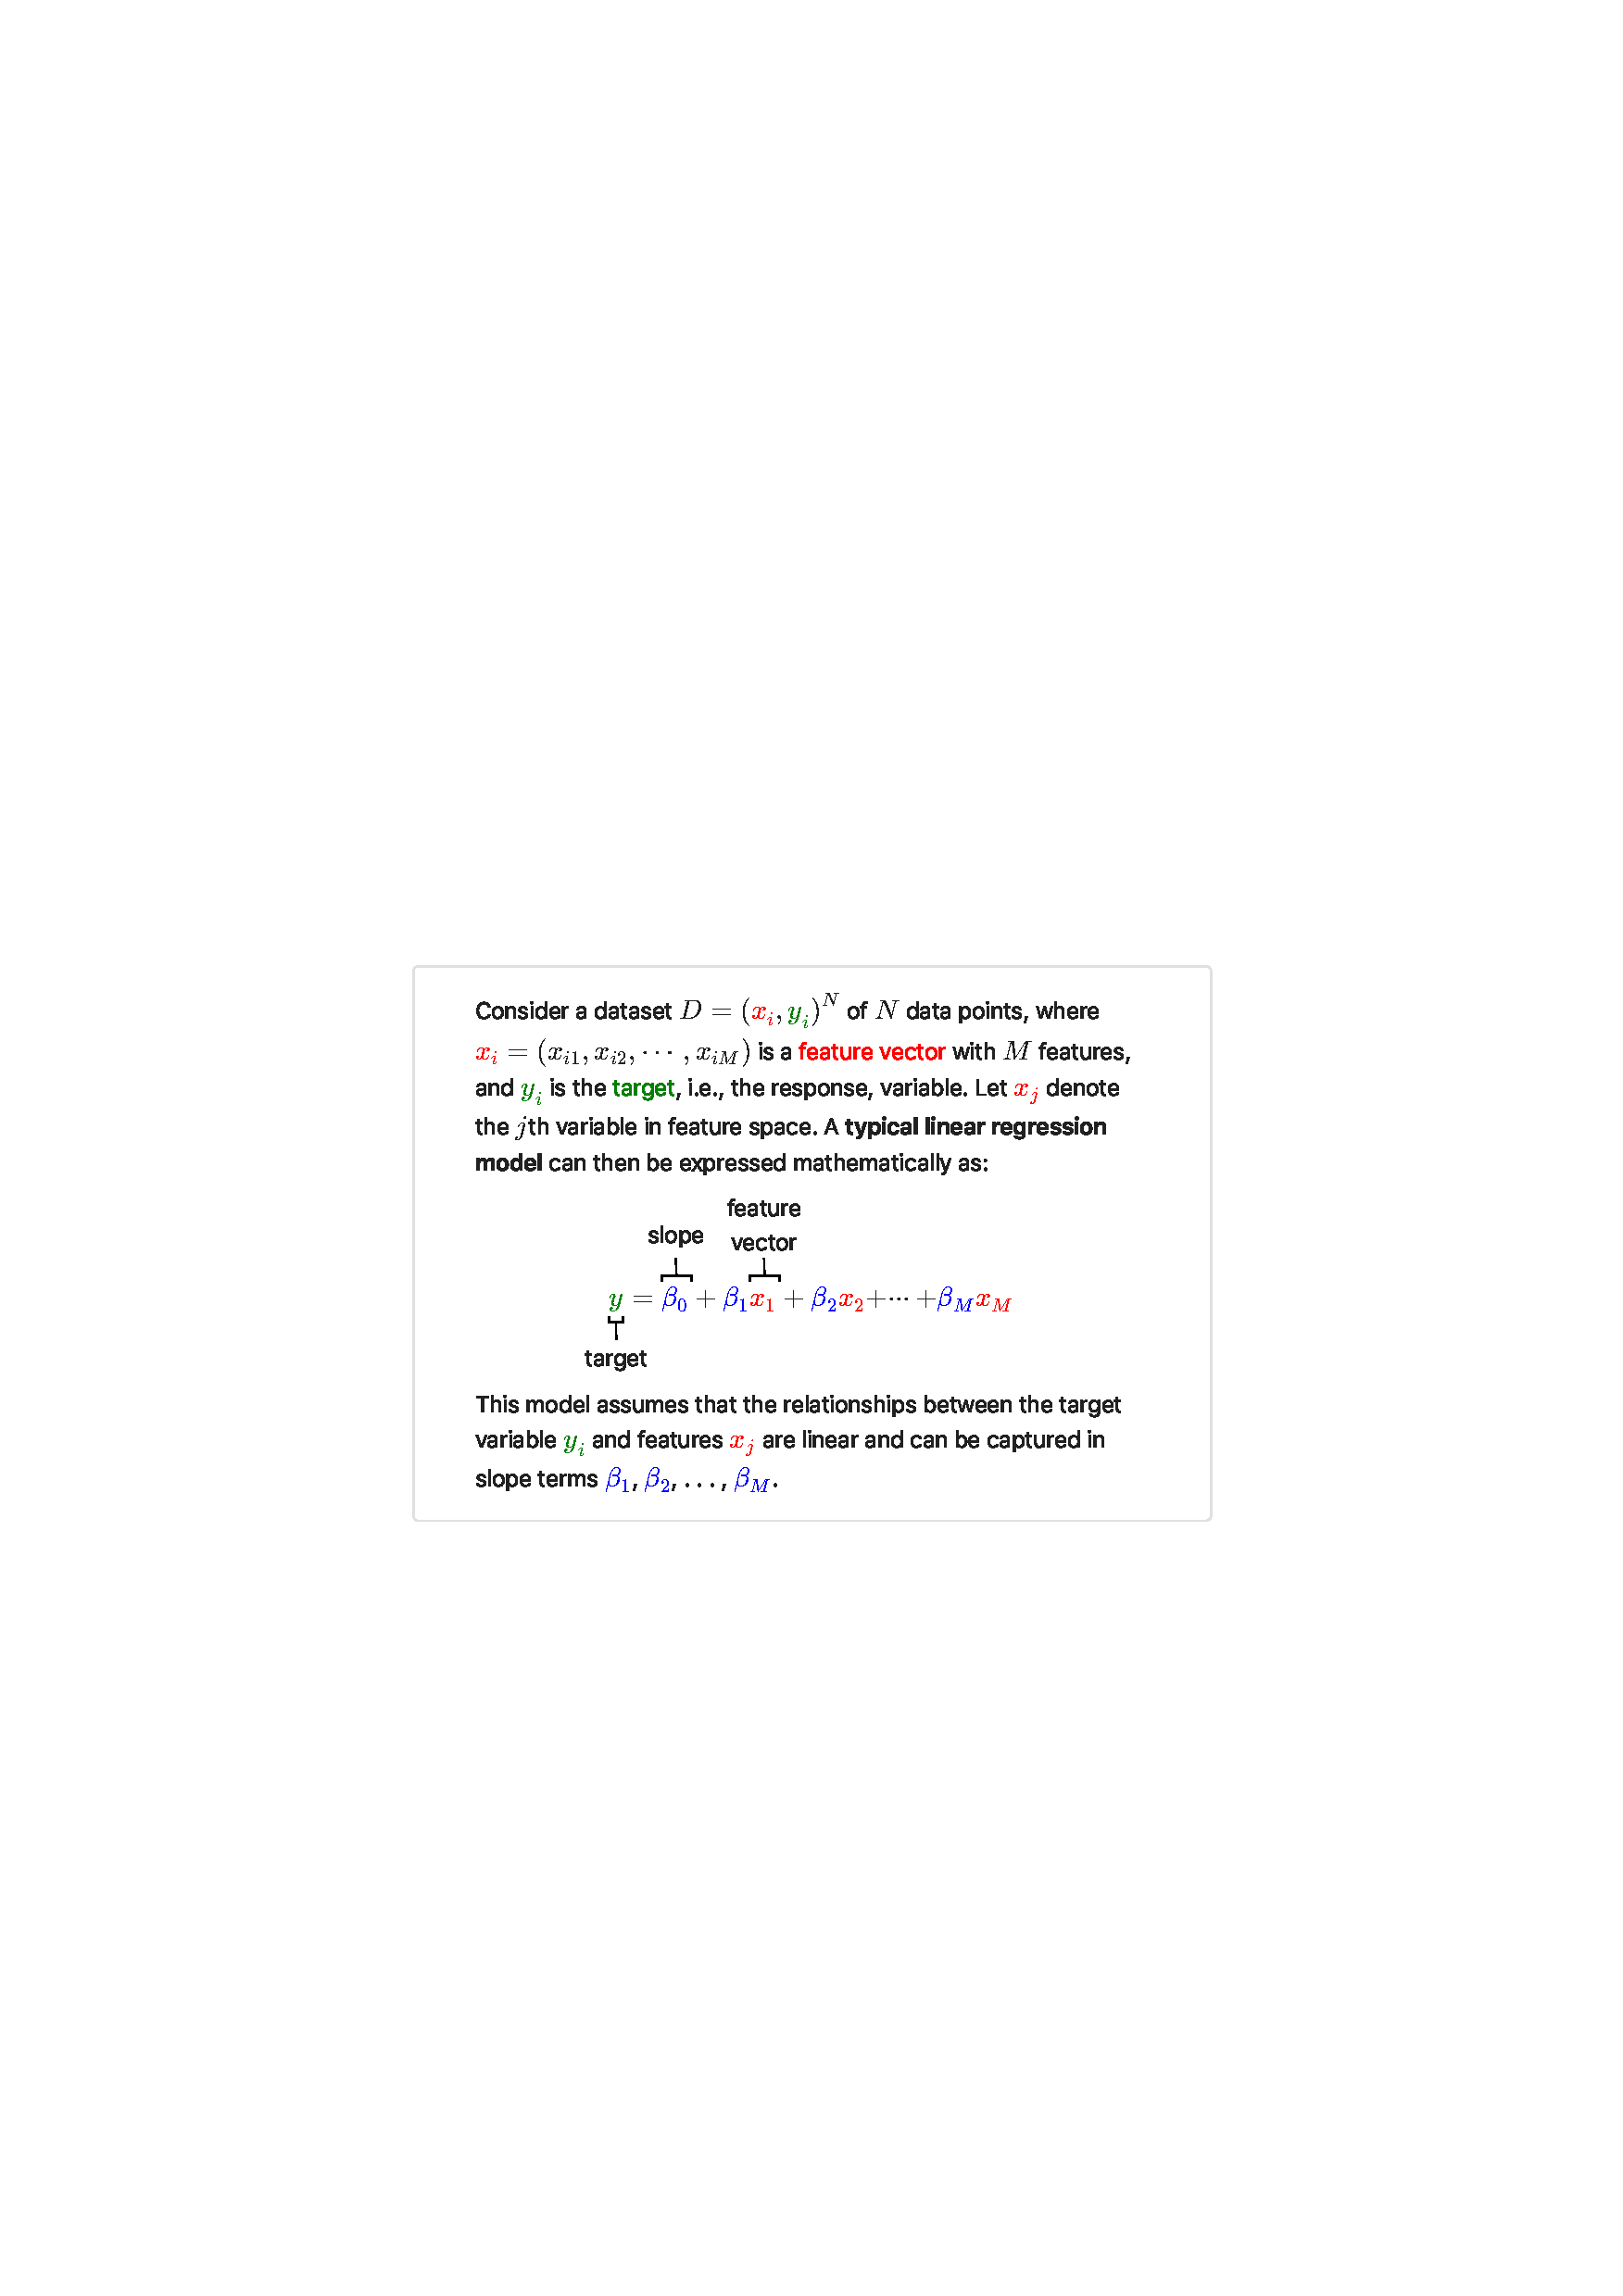
\includegraphics[width=.86\linewidth]{fig/o-2595}\Description{An example augmentation authored by P26 in the exploratory task. All appearances of “x” and “x” with subscripts are colored red, as is the phrase explaining that “x” is a feature vector. All appearances of “y” and “y” with subscripts are colored green, as is the phrase explaining that “y” is the “target” variable. All appearances of “beta” with subscripts are colored in blue. In the block formula, “y” is labeled “target,” “beta-sub-0” is labeled “slope,” and “x-sub-1” is labeled “feature vector,” all with extent markers.}}

Other participants took different approaches. For instance, P13 used labels alone, believing them to be sufficient for a textbook-style passage (and that color was better suited for personal notes):\\[1ex]
{\centerline{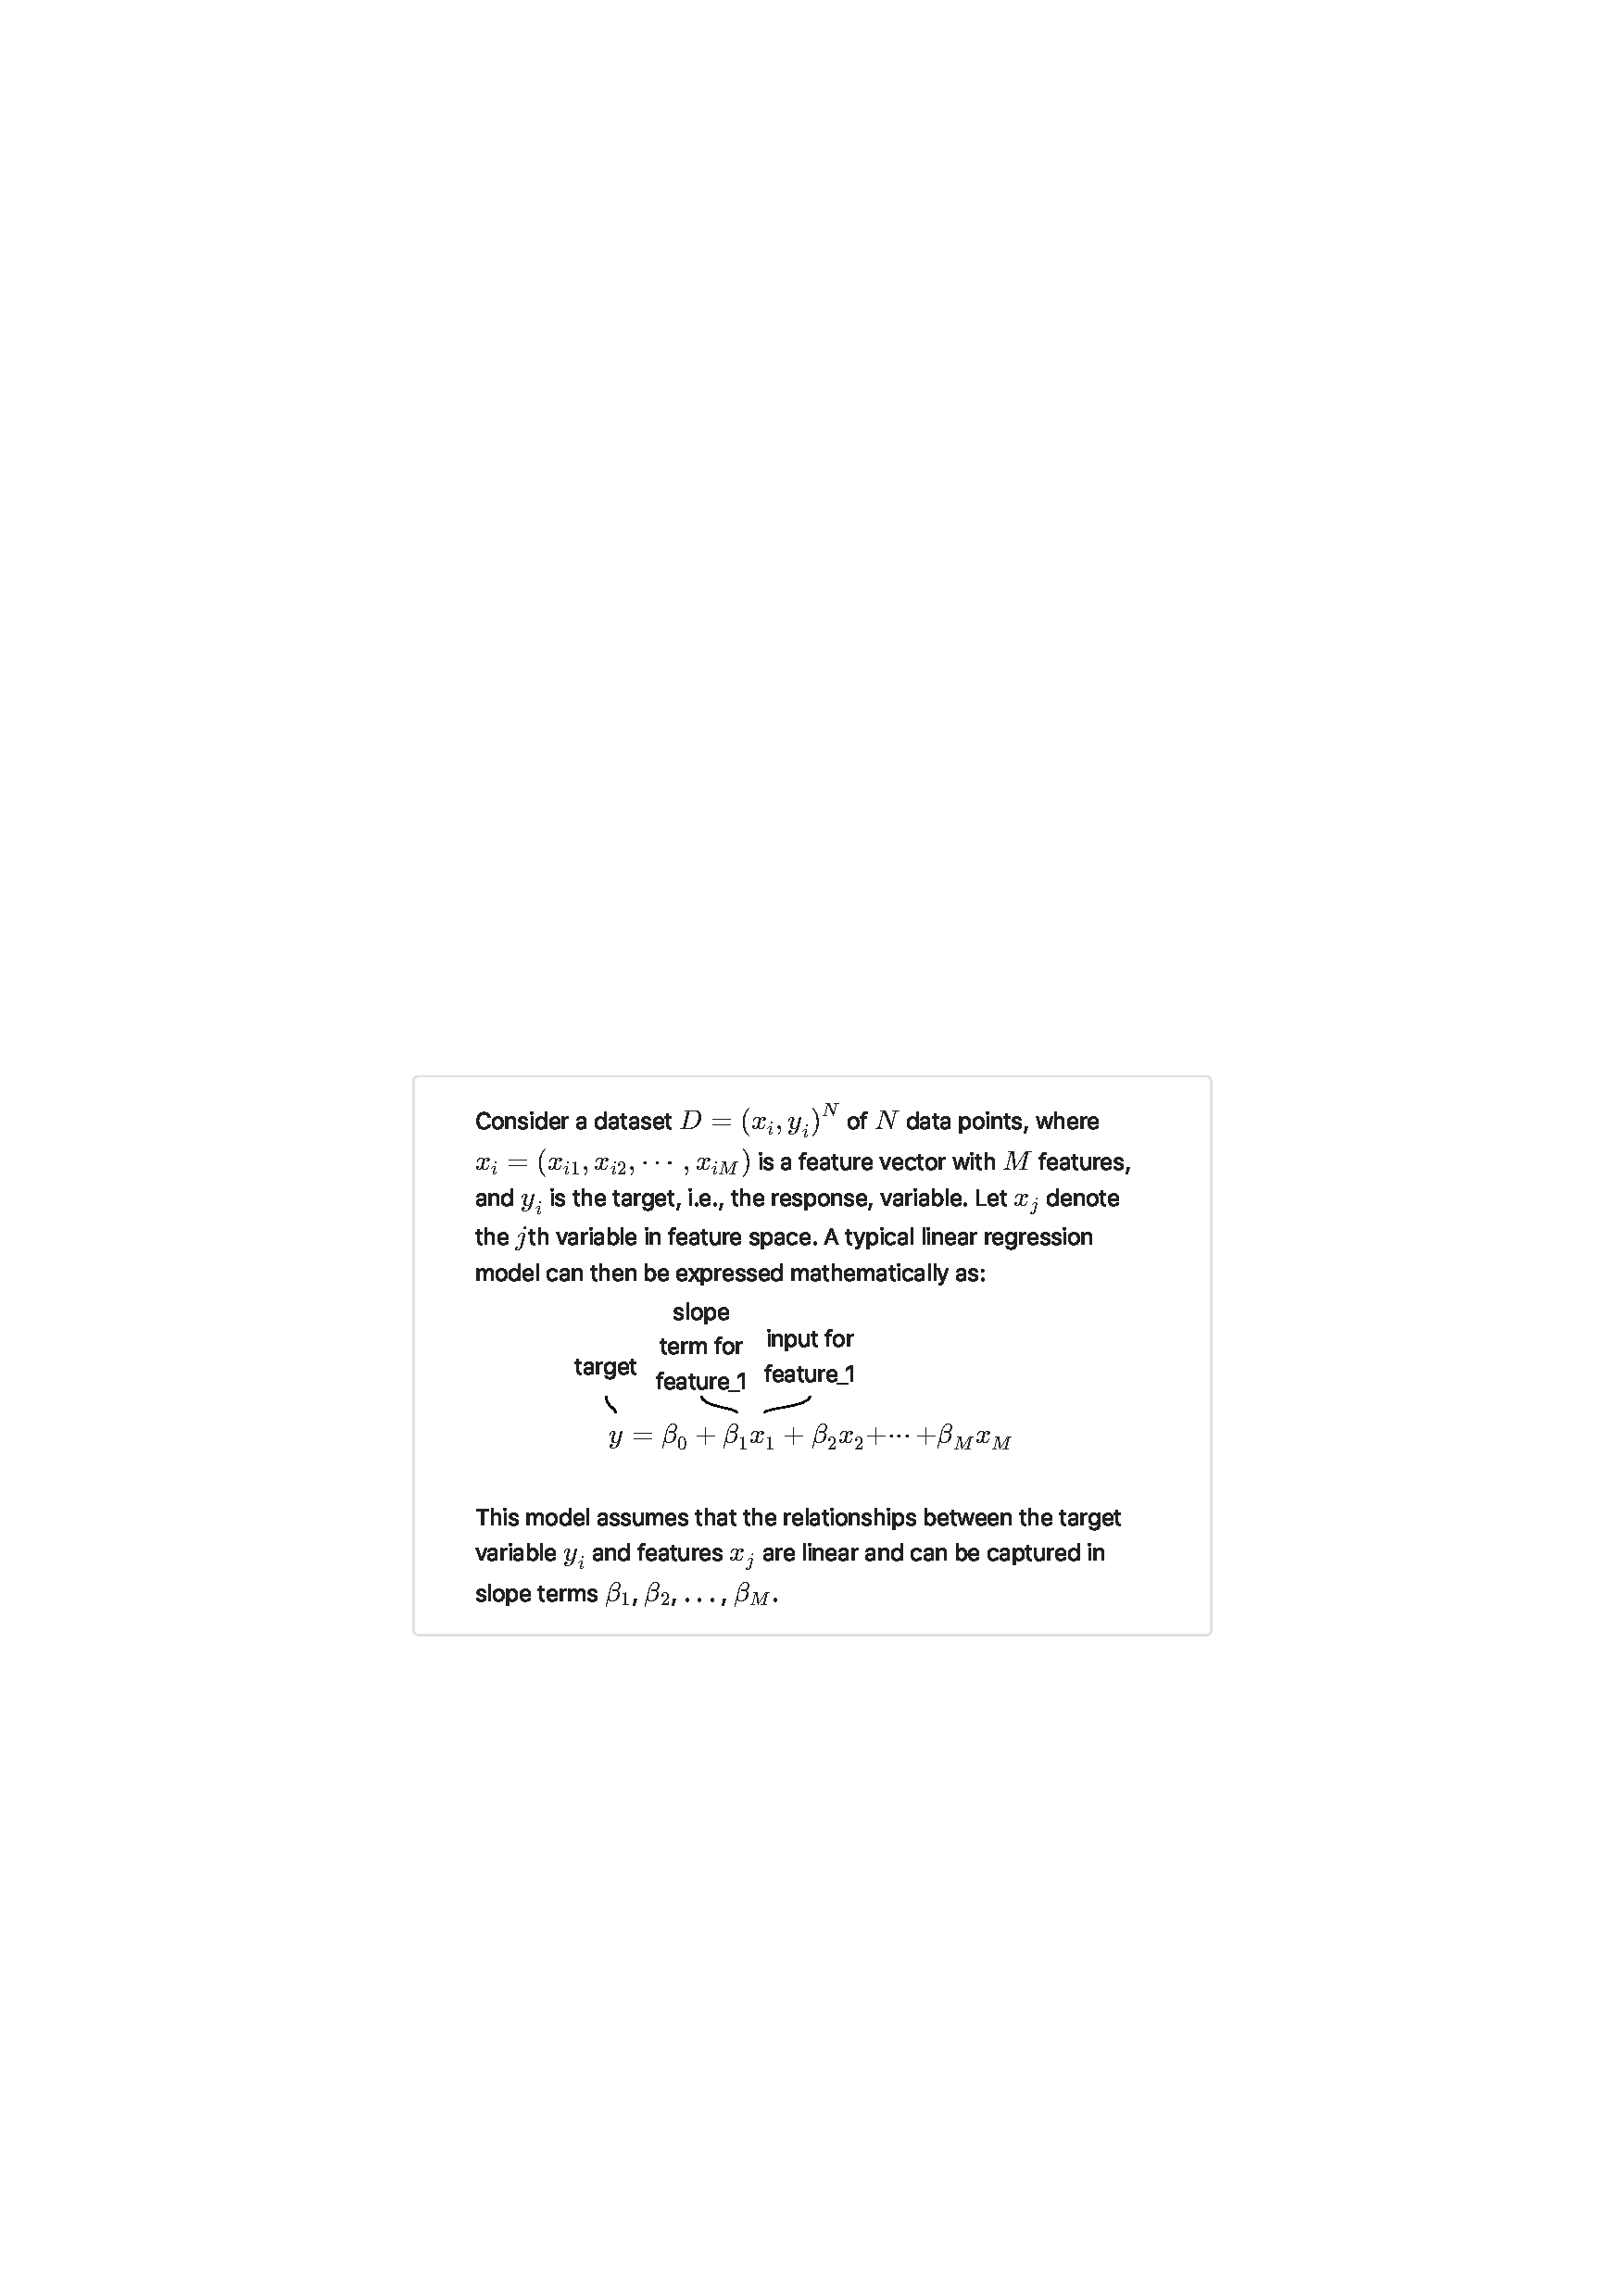
\includegraphics[width=.86\linewidth]{fig/o-3382}\Description{An example augmentation authored by P13 in the exploratory task. Only labels were used. In the block formula, “y” is labeled “target,” “beta-sub-1” is labeled “slope term for feature-underscore-1”; and “x-sub-1” is labeled  “input for feature-underscore-1.” All labels use leader lines, with labels appearing above the formula.}}

Some participants experimented more ambitiously with CSS, when they had sufficient prior knowledge. For instance, P17 experimented with \texttt{background-color}, \texttt{font-size}, and \texttt{font-weight} and expressions, in addition to the other typical augmentations. \\[1ex]
\centerline{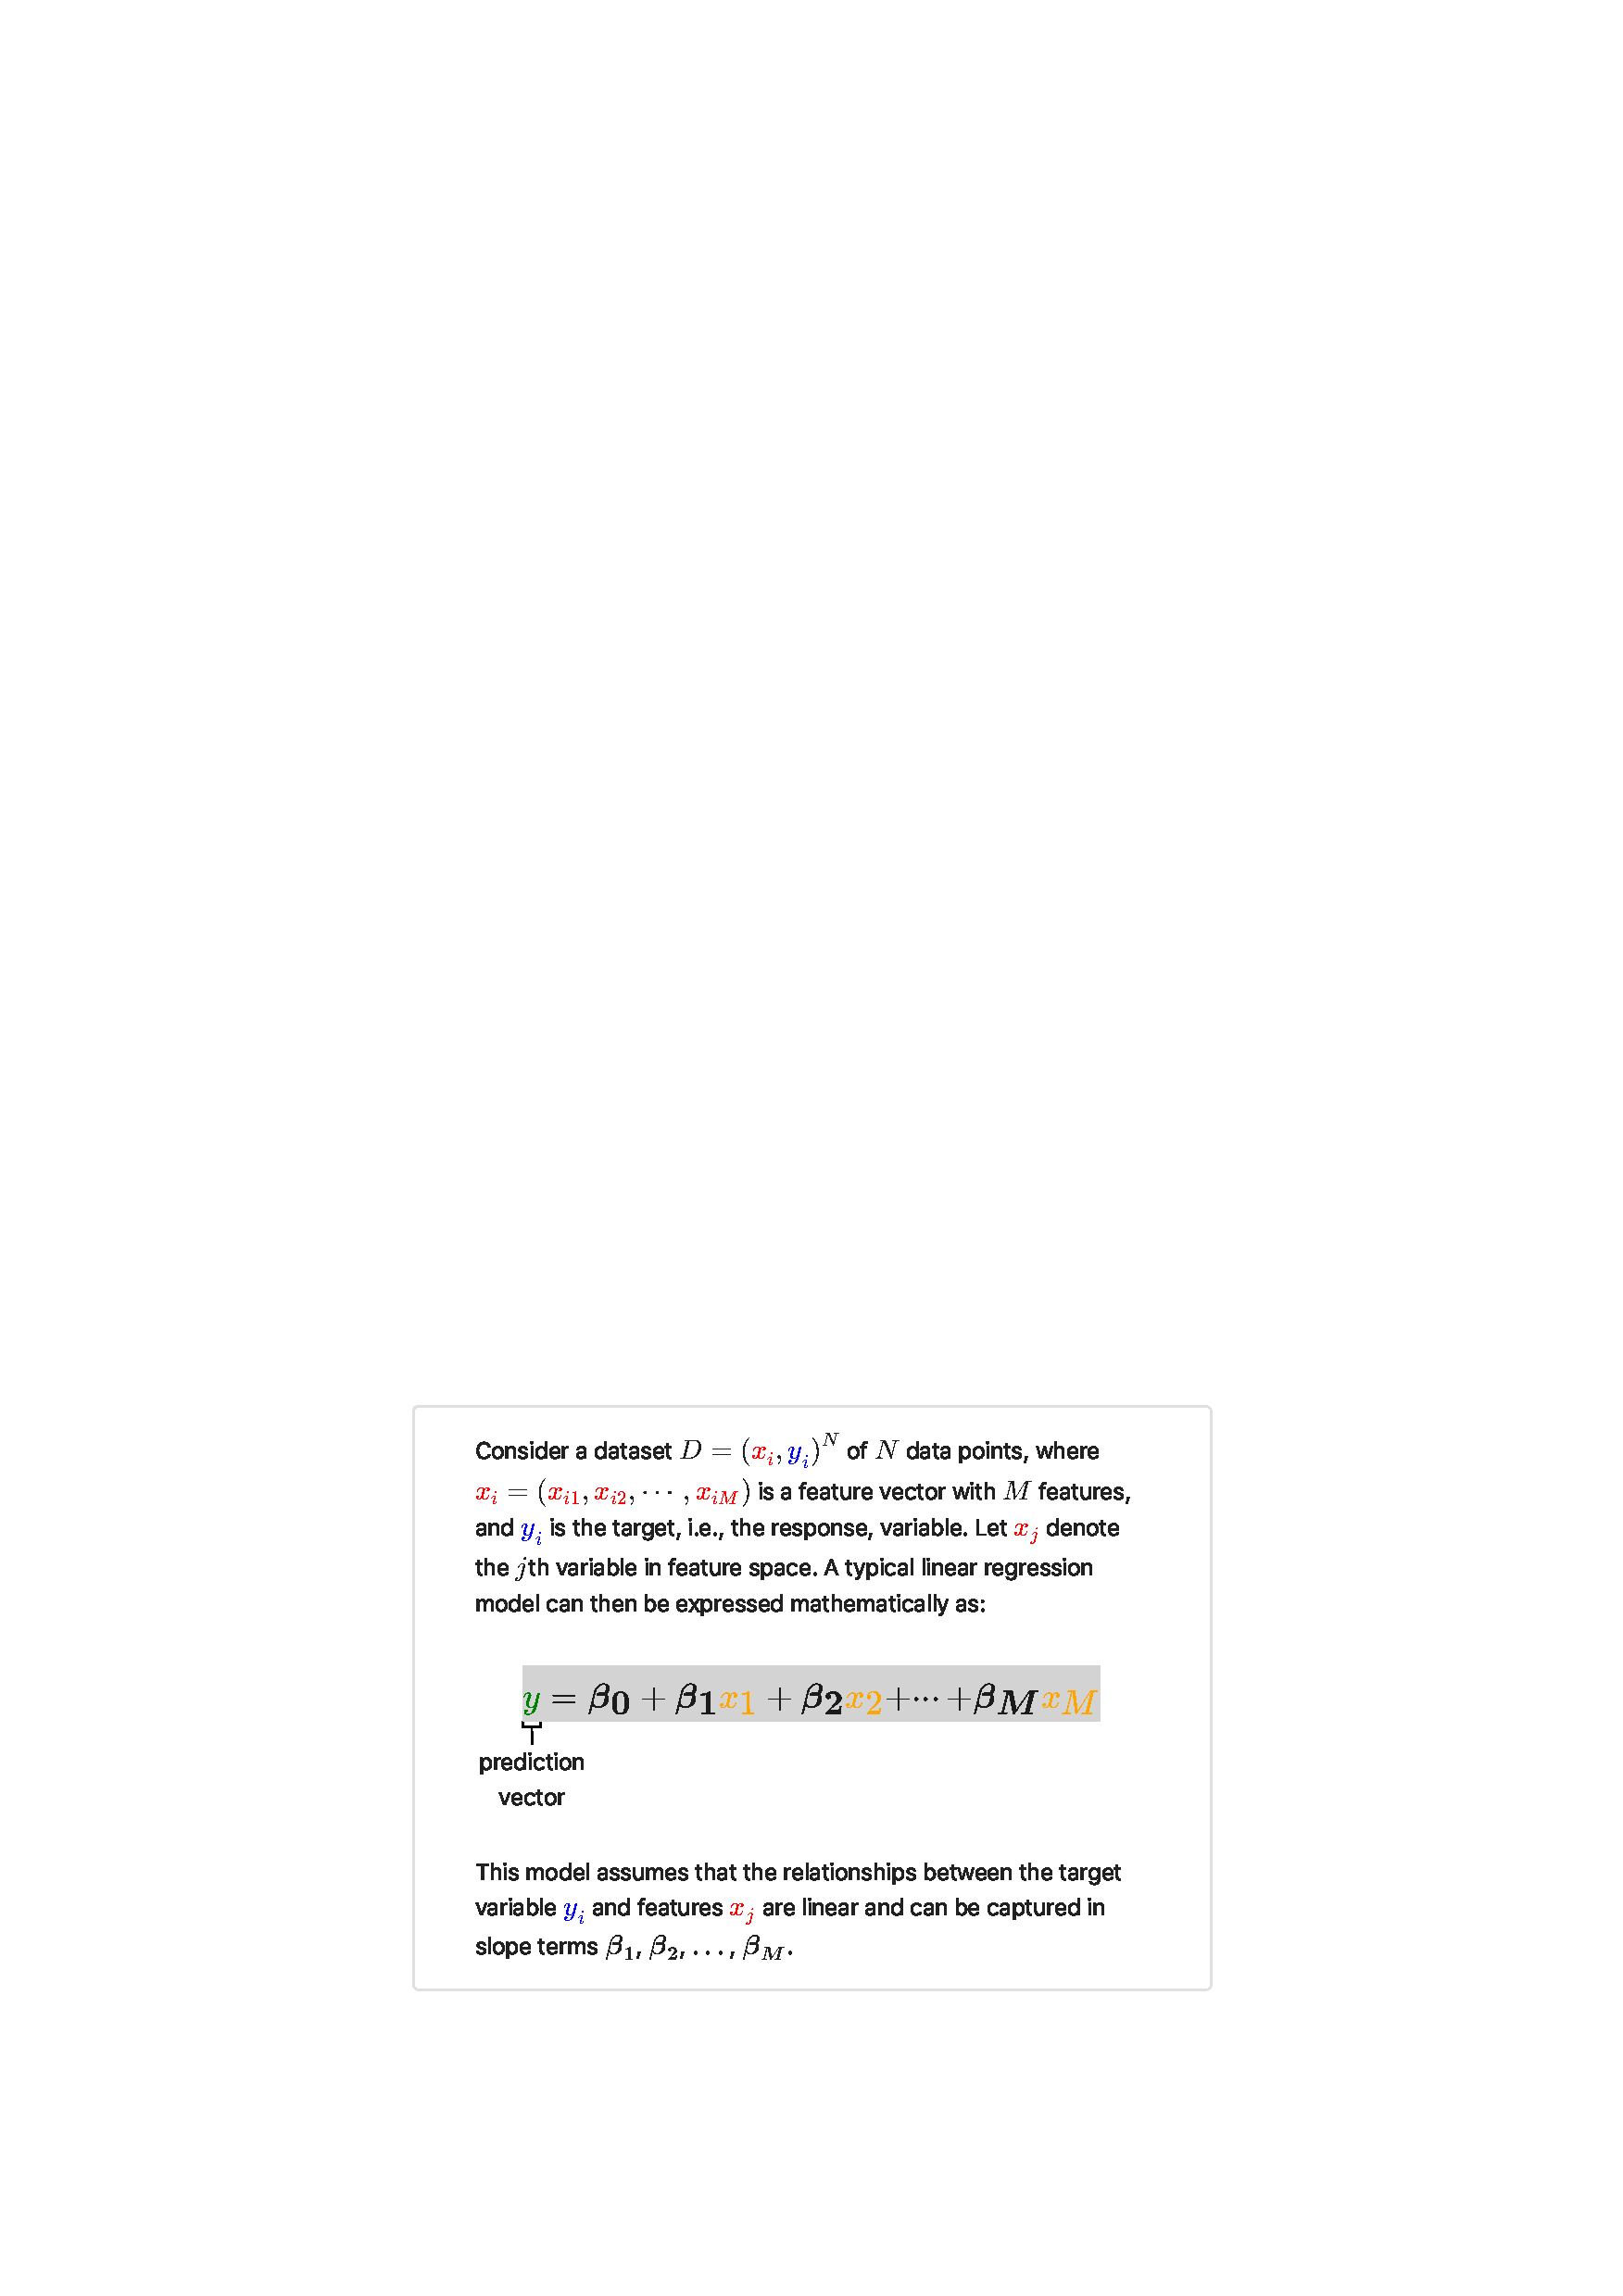
\includegraphics[width=.86\linewidth]{fig/o-3297}\Description{An example augmentation authored by P17 in the exploratory task. All symbols in the block formula are bolded and given a background color of gray. “y” is colored green and given the label “prediction vector.” Outside the formula, all “x” symbols with subscripts are colored red; in the block formula, they are given a gold color.  Outside the formula, all “y” symbols with subscripts are colored in blue. All the “beta” symbols with subscripts are bolded.}}
